This chapter presents the prototypical implementation of the
graph-based DeFi verification concept developed in
Chapter~\ref{chap:concept}. It describes the technologies and
implementation decisions used to realize the proposed architecture,
with particular attention to structured intent processing,
authoritative knowledge acquisition, relationship verification,
and controlled blockchain execution.

The prototype supports Uniswap V3 single-hop ERC-20 swaps and
Aave V3 supply, withdrawal, borrowing, and repayment on Ethereum
Sepolia. The chapter follows the main components of the conceptual
architecture and discusses relevant implementation challenges
and deviations. The correctness, performance, and requirement
fulfilment of the prototype are assessed in
Chapter~\ref{chap:evaluation}.

%############ 4.1  Prototype Overview and Technology Choices  #######
\section{Prototype Overview and Technology Choices}
\label{sec:prototype_overview}

The prototype implements the four main responsibilities
introduced in Section~\ref{sec:overall_system_concept}:
AI-based intent processing, verification knowledge,
relationship verification, and controlled execution.
These responsibilities are realized through a browser-based
demonstration interface, a Python backend, a Neo4j property
graph, and a separate Node.js execution component.
Figure~\ref{fig:prototype_technology_stack} illustrates
the technologies and communication interfaces.

\begin{figure}[htbp]
    \centering
    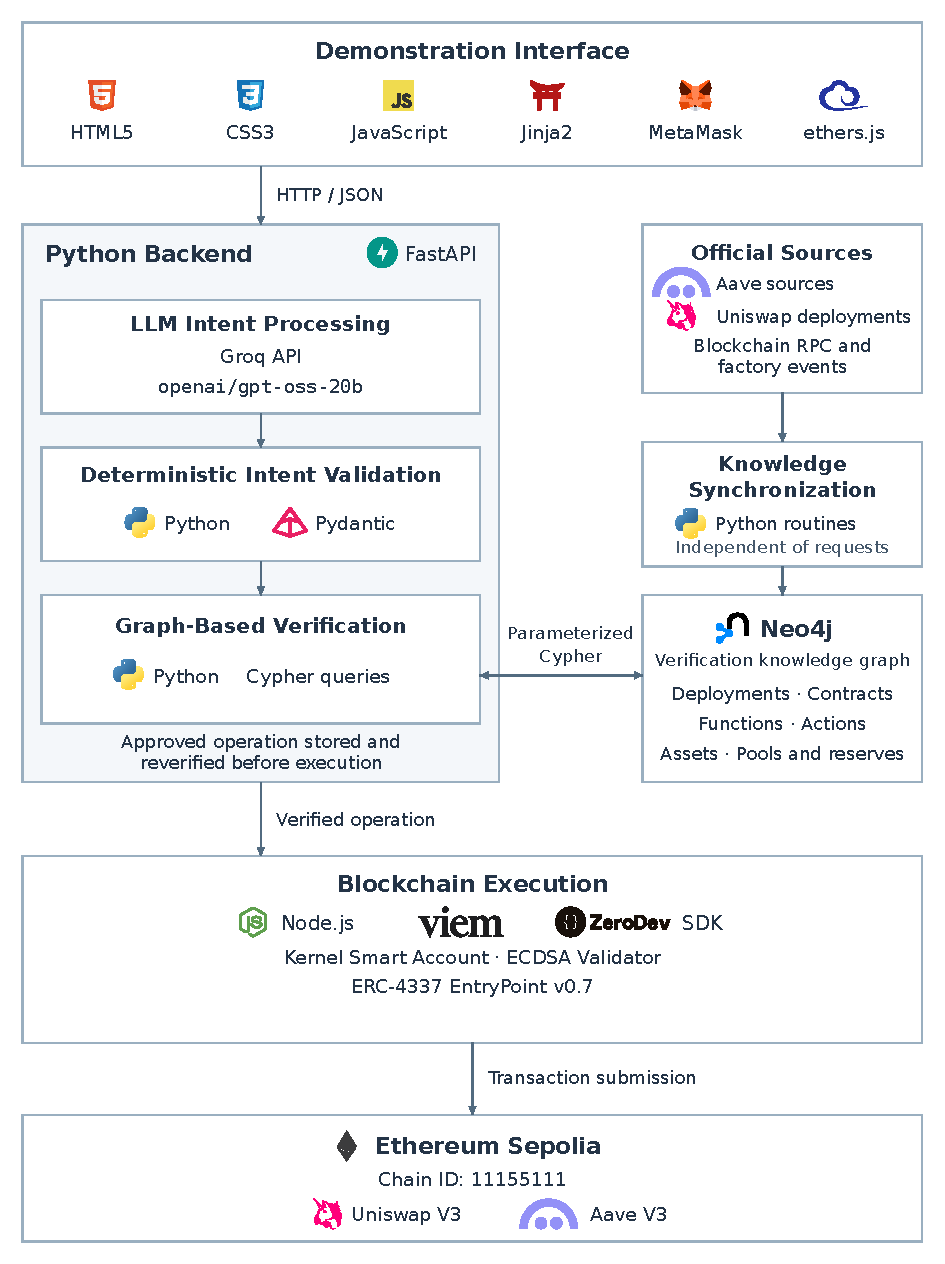
\includegraphics[width=\textwidth]
    {figures/prototype_technology_stack.pdf}
    \caption{Technology stack and communication interfaces
    of the prototype.}
    \label{fig:prototype_technology_stack}
\end{figure}

The demonstration interface is implemented using HTML, CSS,
JavaScript, and Jinja2. It supports natural-language requests,
clarification, verification results, and execution controls.
MetaMask and ethers.js provide browser-wallet connectivity,
while the interface communicates with the backend through
HTTP and JSON. The lightweight design was chosen to keep
the prototype focused on the verification mechanism. The Python backend uses FastAPI and Pydantic to manage API
requests, structured operation models, and the verification
workflow~\cite{implFastAPI,implPydantic}. Intent generation
uses the Groq API with \texttt{openai/gpt-oss-20b}, followed
by deterministic validation. This separation prevents
language-model output from directly determining
execution-critical contract information.

Neo4j was selected because the verification process
requires explicit relationships between protocol
deployments, actions, contracts, functions, and resources.
Parameterized Cypher queries evaluate these connections
against admitted knowledge~\cite{implNeo4jCypher}.
Protocol-specific Python routines acquire and synchronize
this knowledge independently of user requests.

Blockchain interaction is implemented in Node.js using
viem and the ZeroDev SDK. This separates the Python-based
verification logic from the JavaScript smart-account
infrastructure. Execution uses a ZeroDev Kernel smart
account with an ECDSA validator\footnote{In the ZeroDev
Kernel plugin model, a \texttt{sudo} validator provides
unrestricted signing authority, unlike a permission-limited
session-key validator~\cite{implZeroDevPlugins}.}
and ERC-4337 EntryPoint version~0.7
~\cite{implZeroDevSDK,implERC4337}.

Following graph approval, the backend stores the structured
operation and issues an expiring, single-use
\texttt{verification\_id}. Execution retrieves this
operation and repeats graph verification before preparing
the transaction, without reinterpreting the original
request. The implemented authority comparison does not,
however, bind every execution parameter to an immutable
knowledge snapshot. The execution environment is Ethereum Sepolia
(chain ID~11155111). The smart account is controlled by
a backend-configured signer rather than the MetaMask
account connected through the interface. The following
sections describe the implementation of the individual
verification and execution components.


%############ 4.2  LLM-Based Intent Generation  #######

\section{LLM-Based Intent Generation}
\label{sec:llm_intent_generation}

The intent-generation stage implements the language-interpretation
component described in Section~\ref{sec:intent_generation}.
It uses the Groq API with \texttt{openai/gpt-oss-20b} to
convert natural-language requests into candidate structured
intents. The system prompt specifies a JSON representation
containing the action, protocol, input and output assets,
amount, and network. Additional fields capture unsupported
actions, unhandled constraints, and explicitly requested
swap slippage.

The prompt instructs the model to extract information without
introducing assumptions about missing parameters. Unspecified
values are represented as \texttt{null}, while unsupported
operations or conditions should be preserved rather than
silently replaced. For example, ETH must not be substituted
with WETH, and a request mentioning Aave without an action
must not automatically be interpreted as a supply operation.
Contract addresses, functions, and other execution-specific
resources are excluded from the generated intent because
these are resolved through the verification graph. The model is configured with zero temperature, low reasoning
effort, a maximum of 512 completion tokens, and JSON-object
response mode. The latter restricts the response format but
does not enforce a complete intent schema
~\cite{implGroqJSON}. The parser therefore requires a valid
JSON object and retains the expected extraction fields.
Failed model calls or response-parsing attempts are retried
once before an error is returned.

Listing~\ref{lst:generated_intent} illustrates the expected
extraction format for a request to swap 12.375 USDC for WETH
on Uniswap V3 using Ethereum Sepolia with a slippage
tolerance of 0.25\%.

% JSON language definition
\lstdefinelanguage{JSON}{
    morestring=[b]",
    morekeywords={true,false,null},
    sensitive=true,
    showstringspaces=false
}
% Professional JSON listing colors
\definecolor{intentjsonbg}{HTML}{F8FAFC}
\definecolor{intentjsonborder}{HTML}{CBD5E1}
\definecolor{intentjsontext}{HTML}{1E293B}
\definecolor{intentjsonkeyword}{HTML}{1D4ED8}
\definecolor{intentjsonstring}{HTML}{9A3412}
\definecolor{intentjsonnumber}{HTML}{64748B}

% Professional JSON listing style
\lstdefinestyle{intentjson}{
    language=JSON,
    basicstyle=\ttfamily\footnotesize\color{intentjsontext},
    backgroundcolor=\color{intentjsonbg},
    keywordstyle=\color{intentjsonkeyword}\bfseries,
    stringstyle=\color{intentjsonstring},
    numbers=left,
    numberstyle=\ttfamily\tiny\color{intentjsonnumber},
    stepnumber=1,
    numbersep=10pt,
    frame=single,
    framerule=0.5pt,
    rulecolor=\color{intentjsonborder},
    framesep=6pt,
    xleftmargin=2em,
    framexleftmargin=2em,
    xrightmargin=0.5em,
    breaklines=true,
    breakatwhitespace=false,
    columns=fullflexible,
    keepspaces=true,
    showstringspaces=false,
    tabsize=2,
    captionpos=b,
    aboveskip=12pt,
    belowskip=12pt
}

\begin{lstlisting}[
    style=intentjson,
    caption={Illustrative LLM-generated candidate intent for a Uniswap V3 swap.},
    label={lst:generated_intent}
]
{
  "action": "swap",
  "protocol": "Uniswap V3",
  "token_in": "USDC",
  "token_out": "WETH",
  "amount": "12.375",
  "chain": "Ethereum Sepolia",
  "unsupported_action": null,
  "slippage": {
    "value": "0.25",
    "unit": "percent"
  },
  "unhandled_constraints": []
}
\end{lstlisting}


The listing represents the extraction format rather than a
recorded model response. Incomplete requests are processed
using a separate clarification prompt, which receives the
pending candidate, the missing fields, and the user's reply.
The extracted clarification is merged with the existing
candidate and validated again.

The resulting intent remains an untrusted interpretation
of the user's request. Its completeness, supported scope,
and parameter validity are checked by the deterministic
validation component described in
Section~\ref{sec:intent_validation_implementation}.


%############ 4.3  Intent Validation  #######


\section{Intent Validation}
\label{sec:intent_validation_implementation}

The validation stage implements the deterministic checks
described in Section~\ref{sec:intent_validation}. Its main
components are \texttt{llm/normalization.py} and the typed
models in \texttt{core/models.py}. The extracted JSON is
converted into an \texttt{IntentCandidate}, whose fields may
initially be empty to support clarification. Validation
determines whether the candidate represents a complete,
well-formed operation within the supported prototype scope.

Normalization resolves recognized aliases for actions,
protocols, assets, and networks. For example, a deposit
request can be mapped to the Aave supply action. The
supported combinations are Uniswap V3 swaps and Aave V3
supply, withdraw, borrow, and repay operations. Unsupported
actions, protocols, or combinations return
\texttt{UNSUPPORTED} without querying the graph. Amounts are parsed using Python's \texttt{Decimal} type and
must be positive, with no more than 18 fractional decimal
places after removing trailing zeros. Invalid amounts and
swaps with identical normalized input and output assets
produce \texttt{REJECTED}. Recognized Ethereum Sepolia
aliases resolve to chain ID~11155111. An omitted network
uses the configured Sepolia context, whereas an explicitly
different network is unsupported.

For swaps, an explicitly requested slippage tolerance is
converted into basis points\footnote{One basis point (bps)
corresponds to 0.01 percentage points. For example,
100~bps equals 1\%.} and must fall within the supported
range of 1 to 500~bps. When slippage is omitted, the
configured default of 100~bps is applied when preparing
the approved operation. Unsupported conditions, such as
custom recipients, deadlines, and requests containing
multiple operations, prevent further processing rather
than being silently omitted. Additional request-level
checks supplement the model's extraction of such
constraints.

Listing~\ref{lst:required_intent_fields} shows the
action-dependent completeness check implemented in
\texttt{normalization}. Missing information produces
\texttt{NEEDS\_CLARIFICATION} and identifies the fields
required to complete the operation.


% ==================================================
% Professional Python listing style
% ==================================================
\lstdefinestyle{intentpython}{
    language=Python,
    basicstyle=\ttfamily\footnotesize\color{intentjsontext},
    backgroundcolor=\color{intentjsonbg},
    keywordstyle=\color{intentjsonkeyword}\bfseries,
    stringstyle=\color{intentjsonstring},
    commentstyle=\color{intentjsonnumber}\itshape,
    numbers=left,
    numberstyle=\ttfamily\tiny\color{intentjsonnumber},
    stepnumber=1,
    numbersep=10pt,
    frame=single,
    framerule=0.5pt,
    rulecolor=\color{intentjsonborder},
    framesep=6pt,
    xleftmargin=2em,
    framexleftmargin=2em,
    xrightmargin=0.5em,
    breaklines=true,
    breakatwhitespace=false,
    columns=fullflexible,
    keepspaces=true,
    showstringspaces=false,
    tabsize=4,
    captionpos=b,
    aboveskip=12pt,
    belowskip=12pt
}

\begin{lstlisting}[
    style=intentpython,
    caption={Required-field validation and clarification handling.},
    label={lst:required_intent_fields}
]
required = ["action", "protocol", "amount", "token_in"]
if candidate.action == "swap":
    required.append("token_out")

missing = [
    name for name in required
    if getattr(candidate, name) is None
]

if missing:
    friendly = {
        "action": "operation",
        "protocol": "protocol",
        "amount": "amount",
        "token_in": "input asset",
        "token_out": "output asset",
    }

    labels = [friendly[name] for name in missing]

    return IntentResolution(
        status=Decision.NEEDS_CLARIFICATION,
        intent=candidate,
        missing_fields=missing,
        message="Please provide the " + ", ".join(labels) + ".",
        error_code="missing_fields",
    )
\end{lstlisting}


The pending candidate and missing fields are maintained
in process memory by \texttt{pipeline}.
Subsequent clarification responses are merged into the
candidate and validated again. This state has a configurable
expiry but does not survive an application restart.

Successful validation produces an internal
\texttt{APPROVED} status, indicating that the candidate
is ready for graph verification. It does not authorize
execution. Asset symbols are subsequently resolved against
the graph, although the implementation does not explicitly
detect every case of multiple contract addresses sharing
a symbol. Inconsistent capitalization between acquired
Aave symbols and exact-match graph queries may also prevent
a valid asset from being identified. Deterministic
validation therefore establishes structural suitability
without guaranteeing that the extracted intent fully
represents the user's original instruction.


%  #### 4.4 Authoritative Verification Knowledge and Graph Implementation ###

\section{Authoritative Verification Knowledge and Graph Implementation}
\label{sec:verification_knowledge_implementation}

The prototype maintains verification knowledge in a Neo4j
property graph, independently of language-model output and
individual user requests. Protocol-specific acquisition
procedures retrieve deployment and resource information
from external sources, validate the acquired data, and
admit the accepted relationships into the graph. Runtime
verification operates on this maintained representation,
as described in Section~\ref{sec:verification_knowledge}.

\subsection{Knowledge Acquisition and Admission}

The acquisition process distinguishes deployment information,
protocol resources, and callable functions. For Aave V3,
network-specific contract addresses and reserve mappings are
obtained from the official Aave address book
~\cite{implAaveAddressBook}. The acquired information
includes Pool contracts, underlying assets, reserve tokens,
oracles, and interest-rate strategies. Before admission,
the implementation normalizes addresses and checks that
the required contract and asset information is present.

Uniswap V3 deployment information is obtained from the
published deployment records~\cite{implUniswapDeployments}.
The acquisition procedure selects the applicable contracts,
including the factory, swap router, and quoter. It also
queries the blockchain for \texttt{PoolCreated} events,
after checking the RPC network identifier. Event retrieval
is divided into bounded block ranges to accommodate provider
limitations. The resulting records describe pool addresses,
participating tokens, fee tiers, and their creation context.

Discovered pools are not automatically accepted for
verification. The prototype applies a restricted asset
policy under which both pool tokens must belong to an
admitted set consisting of assets represented by active
Aave V3 reserves on the same network and the configured
canonical WETH address. Pools outside this set remain
represented in the graph but are marked as ineligible
for verification. This restriction is a local prototype
policy, not a requirement of the Uniswap protocol.

Callable functions are represented through a configured
interface registry. It associates supported actions with
contract roles, function signatures, and selectors using
the corresponding protocol interfaces
~\cite{implAavePool,implUniswapSingleSwap,implSolidityABI}.
The registry includes Aave lending operations, Uniswap's
\texttt{exactInputSingle} function, and the quoter function
required for swap preparation. Unlike deployment and
resource information, these function mappings are
maintained manually.

\subsection{Implemented Property-Graph Structure}

The graph distinguishes protocol families from their
network-specific deployments. Each deployment is associated
with a \texttt{Chain}, while contracts and tokens are
identified using their network and normalized address.
Selected identifiers are protected by uniqueness constraints,
and Cypher \texttt{MERGE} operations reuse existing graph
entities during synchronization~\cite{implNeo4jCypher}.


Uniswap V3 extends this structure with pools, tokens,
and fee tiers. A deployment connects to its pools through
\texttt{HAS\_POOL}, while \texttt{CREATED\_POOL} records
their factory origin. Token relationships identify the
pool endpoints and participating assets, and fee-tier
relationships preserve the pool configuration.
Figure~\ref{fig:uniswap_graph_implementation}
illustrates a selected subgraph from the implemented
Uniswap V3 verification knowledge. It shows concrete
relationships represented in Neo4j rather than a
complete graph schema. A more detailed reconstruction
of the retrieved graph instance is provided in
Figure~\ref{fig:appendix_uniswap_neo4j}.


\begin{figure}[H]
    \centering
    \resizebox{\linewidth}{!}{%
        

\begingroup
\definecolor{stepfill}{HTML}{F8FAFC}
\definecolor{stepborder}{HTML}{475569}
\definecolor{arrowcol}{HTML}{64748B}
\definecolor{steptext}{HTML}{1E293B}

\begin{tikzpicture}[
    >=stealth,
    graphnode/.style={
        draw=stepborder,
        fill=stepfill,
        text=steptext,
        rounded corners=2pt,
        line width=0.65pt,
        text width=2.67cm,
        minimum height=1.15cm,
        inner xsep=5pt,
        inner ysep=6pt,
        outer sep=0pt,
        align=center,
        font=\sffamily\fontsize{9}{11}\selectfont
    },
    edge/.style={
        ->,
        draw=arrowcol,
        line width=0.76pt,
        rounded corners=0pt,
        shorten <=1pt,
        shorten >=2pt
    },
    rel/.style={
        fill=white,
        text=steptext,
        inner xsep=3pt,
        inner ysep=1.5pt,
        align=center,
        font=\ttfamily\fontsize{7.6}{8.9}\selectfont
    }
]

% --- Top row -----------------------------------------------------
\node[graphnode] (family) at (-5.45,0)
    {\textbf{ProtocolFamily}\\Uniswap V3};
\node[graphnode, text width=3.06cm] (chain) at (5.45,0)
    {\textbf{Chain}\\Ethereum Sepolia\\{\footnotesize chain ID: 11155111}};

% --- Deployment --------------------------------------------------
\node[graphnode, text width=3.72cm] (deployment) at (0,-2.55)
    {\textbf{ProtocolDeployment}\\Uniswap V3 deployment};

% --- Contract layer ---------------------------------------------
\node[graphnode] (router) at (-5.45,-5.0)
    {\textbf{Contract}\\SwapRouter02\\{\footnotesize role: swap\_router}};
\node[graphnode] (factory) at (0,-5.0)
    {\textbf{Contract}\\Uniswap V3 Factory\\{\footnotesize role: factory}};
\node[graphnode] (quoter) at (5.45,-5.0)
    {\textbf{Contract}\\Quoter V2\\{\footnotesize role: quoter}};

% --- Function and pool layer ------------------------------------
\node[graphnode, text width=3.12cm] (execute) at (-5.45,-8.05)
    {\textbf{Function}\\\texttt{exactInputSingle}\\{\footnotesize purpose: execute}\\{\footnotesize selector: \texttt{0x04e45aaf}}};
\node[graphnode] (pool) at (0,-8.05)
    {\textbf{Pool}\\Uniswap V3 pool};
\node[graphnode, text width=4.04cm] (quote) at (5.45,-8.05)
    {\textbf{Function}\\\texttt{quoteExactInputSingle}\\{\footnotesize purpose: preflight}};

% --- Pool resources ---------------------------------------------
\node[graphnode] (token0) at (-2.35,-10.87)
    {\textbf{Token(USDC)}\\Pool token 0 \\{\footnotesize chain ID + address}};
\node[graphnode] (token1) at (2.35,-10.87)
    {\textbf{Token(WETH)}\\Pool token 1 \\{\footnotesize chain ID + address}};

% --- Terminal nodes ---------------------------------------------
\node[graphnode] (action) at (-5.45,-13.45)
    {\textbf{Action}\\\texttt{swap}};
\node[graphnode] (fee) at (0,-13.45)
    {\textbf{FeeTier}\\Pool fee\\configuration};

% --- Top relationships: mirrored orthogonal bends --------------
\draw[edge]
    (family.south) -- (-5.45,-1.36)
    -- node[rel, above, pos=0.50] {HAS\_DEPLOYMENT} (-1.20,-1.36)
    -- ([xshift=-1.20cm]deployment.north);
\draw[edge]
    (chain.south) -- (5.45,-1.36)
    -- node[rel, above, pos=0.50] {HOSTS} (1.20,-1.36)
    -- ([xshift=1.20cm]deployment.north);

% --- Contract ownership: mirrored routing lanes ----------------
\draw[edge]
    ([xshift=-1.47cm]deployment.south) -- (-1.47,-3.58)
    -- node[rel, above, pos=0.51] {DEPLOYED\_CONTRACT} (-5.45,-3.58)
    -- (router.north);
\draw[edge]
    (deployment.south) -- node[rel, left, pos=0.78]
    {DEPLOYED\_CONTRACT} (factory.north);
\draw[edge]
    ([xshift=1.47cm]deployment.south) -- (1.47,-3.58)
    -- node[rel, above, pos=0.49] {DEPLOYED\_CONTRACT} (5.45,-3.58)
    -- (quoter.north);

% --- Pool ownership: dedicated inter-column corridor -----------
\draw[edge]
    ([xshift=0.83cm]deployment.south) -- (0.83,-4.02)
    -- (2.95,-4.02)
    -- node[rel, left, pos=0.54] {HAS\_POOL} (2.95,-8.05)
    -- (pool.east);

% --- Direct contract/function and factory/pool connections ------
\draw[edge]
    (router.south) -- node[rel, left, pos=0.50]
    {EXPOSES\_FUNCTION} (execute.north);
\draw[edge]
    (factory.south) -- node[rel, left, pos=0.50]
    {CREATED\_POOL} (pool.north);
\draw[edge]
    (quoter.south) -- node[rel, right, pos=0.50]
    {EXPOSES\_FUNCTION} (quote.north);

% --- Resource relationships: symmetrical orthogonal bends ------
\draw[edge]
    ([xshift=-0.76cm]pool.south) -- (-0.76,-9.53)
    -- (-2.35,-9.53)
    -- node[rel, left, pos=0.52] {TOKEN0\\SUPPORTS\_TOKEN}
       (token0.north);
\draw[edge]
    ([xshift=0.76cm]pool.south) -- (0.76,-9.53)
    -- (2.35,-9.53)
    -- node[rel, right, pos=0.52] {TOKEN1\\SUPPORTS\_TOKEN}
       (token1.north);
\draw[edge]
    (pool.south) -- node[rel, right, pos=0.77]
    {USES\_FEE\_TIER} (fee.north);

% --- Action relationships: own channels, no node crossings ------
\draw[edge]
    (execute.south) -- node[rel, left, pos=0.58]
    {IMPLEMENTS\_ACTION} (action.north);

\draw[edge]
    (deployment.west) -- node[rel, above, pos=0.47]
    {SUPPORTS\_ACTION} (-8.18,-2.55)
    -- (-8.18,-13.45)
    -- (action.west);

\draw[edge]
    (quote.east) -- (8.22,-8.05)
    -- (8.22,-14.80)
    -- node[rel, above, pos=0.38] {IMPLEMENTS\_ACTION} (-5.45,-14.80)
    -- (action.south);

\end{tikzpicture}
\endgroup
%
    }
    \caption{Selected relationships in the implemented
    Uniswap V3 graph.}
    \label{fig:uniswap_graph_implementation}
\end{figure}

For Aave V3, each lending resource is represented as a
\texttt{Reserve} connected to its deployment through
\texttt{HAS\_RESERVE} and to its underlying asset through
\texttt{UNDERLYING\_ASSET}. Reserve-specific
\texttt{SUPPORTS\_ACTION} relationships describe the
represented lending operations. Additional connections
retain reserve-token, oracle, and interest-rate-strategy
information where available. 
Figure~\ref{fig:aave_graph_implementation}
illustrates the corresponding relationships for
an Aave V3 USDC supply operation. A detailed
reconstruction of the selected graph instance
is provided in Figure~\ref{fig:appendix_aave_neo4j}.


\begin{figure}[H]
    \centering
    \resizebox{\linewidth}{!}{%
        \begingroup
\definecolor{stepfill}{HTML}{F8FAFC}
\definecolor{stepborder}{HTML}{475569}
\definecolor{arrowcol}{HTML}{64748B}
\definecolor{steptext}{HTML}{1E293B}

\begin{tikzpicture}[
  >=stealth,
  graphnode/.style={
    draw=stepborder,
    fill=stepfill,
    text=steptext,
    rounded corners=2pt,
    line width=0.65pt,
    text width=2.78cm,
    minimum height=1.12cm,
    inner xsep=5pt,
    inner ysep=6pt,
    outer sep=0pt,
    align=center,
    font=\sffamily\fontsize{9.4}{11.4}\selectfont
  },
  edge/.style={
    ->,
    draw=arrowcol,
    line width=0.74pt,
    shorten <=1pt,
    shorten >=2pt
  },
  contextedge/.style={
    edge,
    densely dashed
  },
  rel/.style={
    fill=white,
    text=steptext,
    align=center,
    inner xsep=2.5pt,
    inner ysep=1.7pt,
    font=\ttfamily\fontsize{7.7}{9.0}\selectfont
  }
]

% --------------------------------------------------
% Nodes
% --------------------------------------------------

\node[graphnode] (family) at (-5.70,0)
  {\textbf{ProtocolFamily}\\Aave V3};

\node[graphnode,text width=3.00cm] (chain) at (5.70,0)
  {\textbf{Chain}\\Ethereum Sepolia\\
   {\footnotesize chain ID: 11155111}};

\node[graphnode,text width=3.85cm] (deployment)
  at (0,-2.60)
  {\textbf{ProtocolDeployment}\\Aave V3 deployment};

\node[graphnode] (reserve) at (-5.70,-5.35)
  {\textbf{Reserve}\\USDC reserve};

\node[graphnode] (pool) at (5.70,-5.35)
  {\textbf{Contract}\\Aave Pool\\
   {\footnotesize role: pool}};

\node[graphnode] (token) at (-5.70,-8.62)
  {\textbf{Token}\\USDC\\
   {\footnotesize underlying asset}};

\node[graphnode] (action) at (0,-8.62)
  {\textbf{Action}\\\texttt{supply}};

\node[graphnode,text width=3.20cm] (fn)
  at (5.70,-8.62)
  {\textbf{Function}\\\texttt{supply}\\
   {\footnotesize purpose: execute}\\
   {\footnotesize selector: \texttt{0x617ba037}}};

\node[graphnode] (atoken) at (-5.70,-11.85)
  {\textbf{Contract}\\USDC aToken};

\node[graphnode] (debt) at (0,-11.85)
  {\textbf{Contract}\\USDC\\
   {\footnotesize variable-debt token}};

% --------------------------------------------------
% Protocol and chain relationships
% --------------------------------------------------

\draw[edge]
  (family.south) -- (-5.70,-1.42)
  -- node[rel,above,pos=0.49]
     {HAS\_DEPLOYMENT} (-1.15,-1.42)
  -- ([xshift=-1.15cm]deployment.north);

\draw[edge]
  (chain.south) -- (5.70,-1.42)
  -- node[rel,above,pos=0.49]
     {HOSTS} (1.15,-1.42)
  -- ([xshift=1.15cm]deployment.north);

% --------------------------------------------------
% Deployment relationships
% --------------------------------------------------

\draw[edge]
  ([xshift=-1.40cm]deployment.south)
  -- (-1.40,-4.03)
  -- node[rel,above,pos=0.50]
     {HAS\_RESERVE} (-5.70,-4.03)
  -- (reserve.north);

\draw[edge]
  ([xshift=1.40cm]deployment.south)
  -- (1.40,-4.03)
  -- node[rel,above,pos=0.50]
     {DEPLOYED\_CONTRACT} (5.70,-4.03)
  -- (pool.north);

\draw[edge]
  (deployment.south)
  -- node[rel,right,pos=0.58]
     {SUPPORTS\_ACTION}
  (action.north);

% --------------------------------------------------
% Reserve and action relationships
% --------------------------------------------------

\draw[edge]
  (reserve.south)
  -- node[rel,right,pos=0.54]
     {UNDERLYING\_\\ASSET}
  (token.north);

\draw[edge]
  (reserve.east)
  -- (-2.65,-5.35)
  -- node[rel,right,pos=0.50]
     {SUPPORTS\_ACTION} (-2.65,-8.62)
  -- (action.west);

% --------------------------------------------------
% Contract and function relationships
% --------------------------------------------------

\draw[edge]
  (pool.south)
  -- node[rel,right,pos=0.53]
     {EXPOSES\_FUNCTION}
  (fn.north);

\draw[edge]
  (fn.west)
  -- node[rel,above,pos=0.49]
     {IMPLEMENTS\_\\ACTION}
  (action.east);

% --------------------------------------------------
% Supplementary reserve-token relationships
% Dashed edges distinguish contextual graph knowledge.
% --------------------------------------------------

% Reserve -> aToken
\draw[contextedge]
    ([yshift=-4pt]reserve.west)
    -| (-8.12,-11.85)
    -- (atoken.west);

\node[rel, rotate=90]
    at (-8.12,-8.55)
    {HAS\_A\_TOKEN};

% Reserve -> variable-debt token
\draw[contextedge]
    ([yshift=4pt]reserve.west)
    -| (-9.05,-13.28)
    -- node[rel,above,pos=0.46]
       {HAS\_VARIABLE\_DEBT\_TOKEN}
       (0,-13.28)
    -- (debt.south);

% aToken -> underlying asset
\draw[contextedge]
  (atoken.north)
  -- node[rel,right,pos=0.53]
     {REPRESENTS\_\\ASSET}
  (token.south);

% Variable-debt token -> underlying asset
\draw[contextedge]
  (debt.west)
  -- node[rel,above,pos=0.50]
     {DEBT\_FOR} (-3.33,-11.85)
  -- (-3.33,-8.62)
  -- (token.east);

\end{tikzpicture}
\endgroup
%
    }
    \caption{Selected relationships in the implemented
    Aave V3 graph for USDC supply.}
    \label{fig:aave_graph_implementation}
\end{figure}




% ==================================================
% Cypher language definition
% ==================================================
\lstdefinelanguage{Cypher}{
    morekeywords={
        MATCH,OPTIONAL,WHERE,WITH,RETURN,AS,
        AND,OR,NOT,ORDER,BY,LIMIT,MERGE,
        SET,CREATE,DELETE,DETACH,DISTINCT,
        UNWIND,CALL,YIELD,REMOVE,ON,
        CASE,WHEN,THEN,ELSE,END,IN
    },
    sensitive=false,
    morecomment=[l]{//},
    morestring=[b]',
    morestring=[b]"
}

% ==================================================
% Professional Cypher listing colors
% ==================================================
\definecolor{cypherbg}{HTML}{F8FAFC}
\definecolor{cypherborder}{HTML}{CBD5E1}
\definecolor{cyphertext}{HTML}{1E293B}
\definecolor{cypherkeyword}{HTML}{1D4ED8}
\definecolor{cypherstring}{HTML}{9A3412}
\definecolor{cypherlineno}{HTML}{64748B}

% ==================================================
% Professional Cypher listing style
% ==================================================
\lstdefinestyle{thesiscypher}{
    language=Cypher,
    basicstyle=\ttfamily\footnotesize\color{cyphertext},
    backgroundcolor=\color{cypherbg},
    keywordstyle=\color{cypherkeyword}\bfseries,
    stringstyle=\color{cypherstring},
    commentstyle=\color{cypherlineno}\itshape,
    numbers=left,
    numberstyle=\ttfamily\tiny\color{cypherlineno},
    stepnumber=1,
    numbersep=10pt,
    frame=single,
    framerule=0.5pt,
    rulecolor=\color{cypherborder},
    framesep=6pt,
    xleftmargin=2em,
    framexleftmargin=2em,
    xrightmargin=0.5em,
    breaklines=true,
    columns=fullflexible,
    keepspaces=true,
    showstringspaces=false,
    captionpos=b
}

\begin{lstlisting}[
    style=thesiscypher,
    caption={Selected Cypher statements for protocol deployment construction (abridged).},
    label={lst:deployment_graph_construction}
]
MERGE (chain:Chain {chain_id: $chain_id})
MERGE (family:ProtocolFamily {key: $protocol_key})
MERGE (deployment:ProtocolDeployment {key: $deployment_key})

SET deployment.chain_id = $chain_id,
    deployment.source_url = $source_url,
    deployment.graph_version = $graph_version,
    deployment.last_synced_at = $synced_at

MERGE (family)-[:HAS_DEPLOYMENT]->(deployment)
MERGE (chain)-[:HOSTS]->(deployment)
MERGE (deployment)-[:DEPLOYED_ON]->(chain)
\end{lstlisting}


Listing~\ref{lst:deployment_graph_construction}
illustrates how protocol deployments are connected to
their protocol families and blockchain networks.
Source references and synchronization timestamps
are retained as deployment properties.


The shared execution structure connects a deployment to
its supported actions through \texttt{SUPPORTS\_ACTION}
and to its contracts through \texttt{DEPLOYED\_CONTRACT}.
Contracts expose callable functions through
\texttt{EXPOSES\_FUNCTION}, while
\texttt{IMPLEMENTS\_ACTION} identifies the action
associated with each function. Contract roles and active
states are retained on the relevant relationships.

These protocol-specific structures preserve the relationships
needed to establish execution context. The figures present
selected stored relationships; the action-specific Cypher
queries in the following section determine which of these
relationships participate in verification.
Listing~\ref{lst:deployment_graph_construction}
illustrates the construction of a protocol deployment
and its relationship to the corresponding protocol
family and blockchain network. Source references and
synchronization timestamps are stored as properties
of the deployment.

\subsection{Synchronization, Freshness, and Implementation Limits}

Knowledge synchronization follows three stages:
acquisition, validation, and admission. Each protocol
deployment can be synchronized independently through
a command-line workflow. The source information is
retrieved and validated before existing deployment
relationships are updated. This prevents failed acquisition
from immediately replacing previously admitted knowledge. Synchronization outcomes are recorded through
\texttt{KnowledgeSource} nodes and
\texttt{SYNCHRONIZED\_FROM} relationships. The stored
information includes source references, synchronization
status, timestamps, and failure details. During successful
admission, applicable existing relationships are marked
inactive and those present in the accepted data are
reactivated. Historical graph entities can therefore
remain available without necessarily supporting new
verification approvals.

The verifier evaluates knowledge freshness using the most
recent successful synchronization timestamp, with a
configurable maximum age of 168 hours by default.
Unsuccessful synchronization attempts do not automatically
invalidate previously accepted information while that
information remains within the permitted age. Coverage
properties, including \texttt{pool\_discovery\_complete}
and \texttt{asset\_coverage}, indicate the scope of the
acquired data. They do not establish complete knowledge
of all protocol resources.

The synchronization process is invoked explicitly and
does not include a background scheduler or automatic
source-change monitoring. Furthermore, graph admission
consists of multiple database operations rather than
an atomic replacement of the entire deployment. A failure
during admission or a concurrent verification request
can therefore encounter a partially updated graph. Additional limitations concern the admission policies.
Uniswap pool eligibility depends partly on Aave reserve
information already stored in the graph, without an
independent freshness check of that dependency during
admission. For Aave, supply and withdrawal relationships
are inferred from parsed reserves, while borrowing and
repayment relationships depend on the presence of a
variable-debt token. The loader does not examine live
pause, freeze, or borrowing-enabled settings, and obsolete
reserve-action relationships are not comprehensively
removed.

Consequently, the graph represents admitted execution
relationships and their synchronization context, but
does not establish every aspect of current protocol
availability. It also does not preserve an immutable
knowledge snapshot for each verification. These limits
are considered when interpreting the verification
decisions described in the following section.


% ## 4.5 Relationship Verification and Decision  ##

\section{Relationship Verification and Decision}
\label{sec:relationship_verification_implementation}

The verifier implements the action-specific relationship checks
defined in Section~\ref{sec:relationship_verification} through
parameterized Cypher queries. It receives the normalized protocol,
action, assets, and chain identifier. The amount and slippage
parameters are retained for execution preparation but do not
participate in the graph queries. Verification is performed against
the admitted knowledge described in
Section~\ref{sec:verification_knowledge_implementation}.

\subsection{Action-Specific Relationship Verification}

For Uniswap V3, the verifier requires a deployment
supporting the swap action, an active and eligible
liquidity pool connecting the requested assets, and
verified router and quoter contracts exposing the
corresponding functions. These relationships must
match within the same deployment and network context.
The query returns contract addresses, function
information, pool fees, and token properties required
for execution preparation. Matching routes are ordered
by their recorded attributes rather than quoted prices.

Aave V3 follows a different relationship pattern because
lending operations depend on reserves rather than
liquidity pools. The verifier requires an active reserve
linked to the requested underlying asset, action support
from both the reserve and deployment, and a verified Pool
contract exposing the corresponding lending function.
The query returns the contract, asset, and function
information required for transaction preparation.

In both cases, verification checks connected relationships
rather than the independent existence of contracts and
assets. The complete parameterized Cypher queries are
provided in Appendix~\ref{app:runtime_verification_queries}.

Although both protocols use the same verification pipeline,
their implementations differ in knowledge acquisition,
graph relationships, and transaction preparation.
Table~\ref{tab:protocol_implementation_differences}
summarizes these differences and the components that
would need adaptation when supporting additional protocols.

\begin{table}[htbp]
\centering
\begingroup
\small
\renewcommand{\arraystretch}{1.18}
\caption{Protocol-specific implementation differences.}
\label{tab:protocol_implementation_differences}

\begin{tabular}{
    @{}
    p{0.21\linewidth}
    p{0.33\linewidth}
    p{0.33\linewidth}
    @{}
}
\hline
\textbf{Aspect} &
\textbf{Uniswap V3} &
\textbf{Aave V3} \\
\hline

Supported actions &
Swap &
Supply, withdraw, borrow, repay \\

Main resource &
Liquidity pool &
Lending reserve \\

Execution contracts &
SwapRouter02 and Quoter V2 &
Aave Pool \\

Required relationships &
Deployment, action, pool, assets, router, quoter,
and callable functions &
Deployment, action, reserve, underlying asset,
Pool contract, and callable function \\

Supporting graph data &
Factory origin, token positions, and fee tiers &
aToken and variable-debt token associations \\

Knowledge acquisition &
Deployment records and factory events &
Address-book and reserve information \\

Execution preparation &
Route quotation, slippage, balances,
and token allowances &
Lending calldata, balances, and
action-specific allowances \\

Extension requirements &
Pool discovery, routing, quoting,
and swap interfaces &
Reserve models, lending actions,
and protocol-specific interfaces \\

\hline
\end{tabular}
\endgroup
\end{table}


\subsection{Verification Decisions and Traceability}

Before evaluating the relationship patterns, the verifier
checks the availability and freshness of the applicable
knowledge. The most recent successful synchronization
timestamp is compared with a configurable age limit,
which defaults to 168 hours. Missing deployment information,
stale knowledge, or unavailable graph access prevents
approval and produces \texttt{INSUFFICIENT\_EVIDENCE}. A matching relationship pattern in fresh admitted knowledge
can produce \texttt{APPROVED}. When no matching path exists,
the verifier distinguishes an unsupported relationship
from incomplete knowledge. If the applicable coverage
indicator records sufficient completeness, the result is
\texttt{REJECTED}. Otherwise, the verifier returns
\texttt{INSUFFICIENT\_EVIDENCE}.

For Uniswap, the completeness assessment uses the recorded
pool-discovery indicator. For Aave, it uses the declared
address-book asset coverage. These indicators describe the
scope of locally synchronized knowledge rather than proving
universal protocol completeness. A positive relationship
match does not require exhaustive coverage of all protocol
resources. Requests outside the supported scope return
\texttt{UNSUPPORTED} before relationship matching. The verification result contains the decision, normalized
operation context, and resolved execution information or
an explanatory failure reason. 

Verification latency is
recorded separately from language-model interpretation and
blockchain submission. For unsuccessful outcomes, the implementation can also
produce structured diagnostic information. This includes
rule identifiers, relevant entities or relationships, and
expected and observed conditions where the available
evidence permits localization. Source, freshness, and
coverage information provide context for interpreting
the failure. These diagnostics are constructed through
deterministic checks rather than generated by the language
model.

Diagnostic inspection is bounded and does not necessarily
identify a unique cause. A failure may remain
\texttt{not\_localized}, or diagnostics may be
\texttt{unavailable}. Neither condition changes the
original verification decision.

Figures~\ref{fig:verification_result} and
\ref{fig:verification_rejection} illustrate the approved
and rejected outcomes presented through the prototype
interface.

\begin{figure}[H]
    \centering
    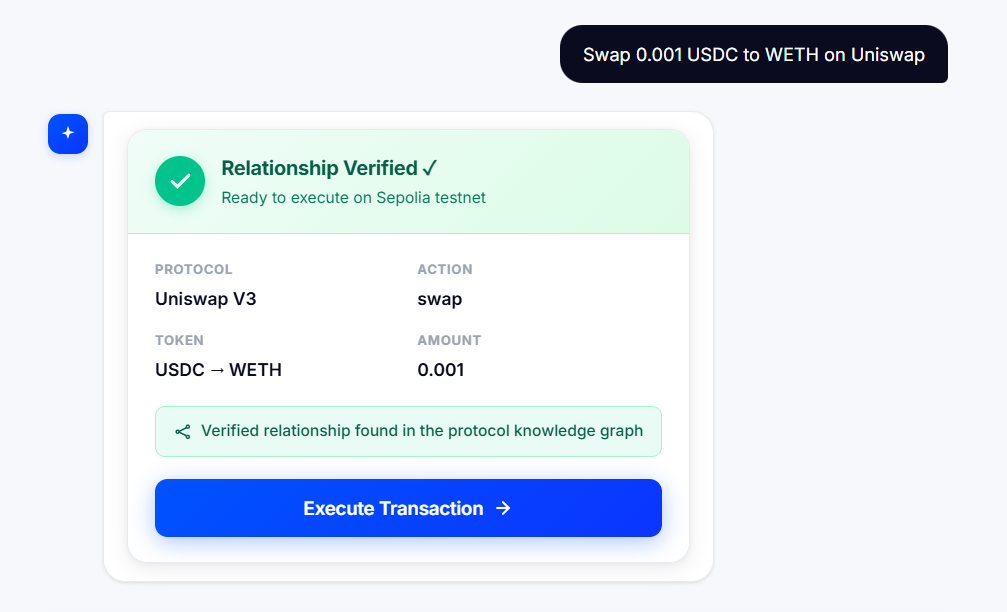
\includegraphics[width=0.90\linewidth]
        {figures/verification_result.png}
    \caption{Approved Uniswap V3 swap displayed before
    blockchain submission.}
    \label{fig:verification_result}
\end{figure}

An approved result establishes consistency with the
represented execution relationships within the admitted
knowledge context. It does not guarantee transaction
success, economic safety, or the absence of smart-contract
vulnerabilities. The returned information also does not
constitute a complete, immutable record of every verified
relationship.
\begin{figure}[H]
    \centering
    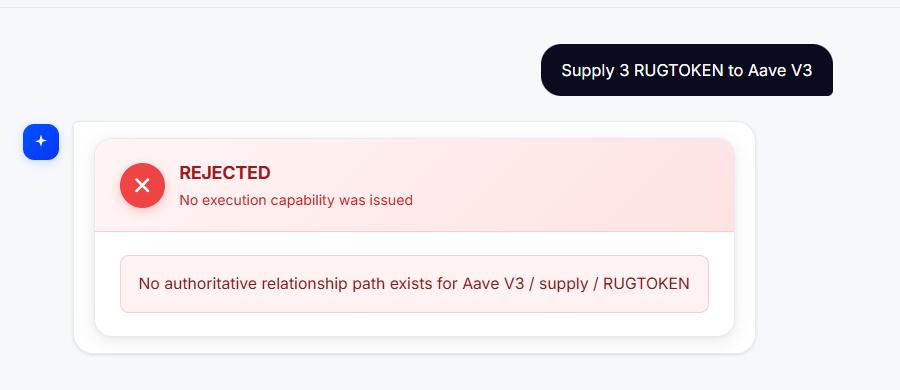
\includegraphics[width=0.85\linewidth]
        {figures/verification_result_failure.png}
    \caption{Rejected Aave V3 supply request for
    \texttt{RUGTOKEN}, without execution authorization.}
    \label{fig:verification_rejection}
\end{figure}


Following approval, the backend retains the structured
operation and creates an expiring verification identifier.
The controlled handover to smart-wallet execution is
described in the following section.


% % #### 4.6 Controlled Smart-Wallet Execution ###
\section{Controlled Smart-Wallet Execution}
\label{sec:controlled_execution_implementation}


After reviewing the approved operation, the user can
initiate execution through the demonstration interface.
This confirmation triggers the execution request but does
not constitute cryptographic authorization by the connected
MetaMask account. 




\begin{figure}[H]
    \centering
    \resizebox{0.95\linewidth}{!}{%
        % \begingroup
% \definecolor{stepfill}{HTML}{F8FAFC}
% \definecolor{stepborder}{HTML}{475569}
% \definecolor{arrowcol}{HTML}{64748B}
% \definecolor{steptext}{HTML}{1E293B}

% \begin{tikzpicture}[
%     >=stealth,
%     execbox/.style={
%         draw=stepborder,
%         fill=stepfill,
%         text=steptext,
%         rounded corners=2pt,
%         line width=0.6pt,
%         text width=6.2cm,
%         minimum height=1.6cm,
%         inner xsep=8pt,
%         inner ysep=6pt,
%         align=center,
%         font=\sffamily\linespread{1}\fontsize{10}{12}\selectfont,
%         execute at begin node={
%             \hyphenpenalty=10000
%             \exhyphenpenalty=10000
%         }
%     },
%     execarrow/.style={
%         ->,
%         draw=arrowcol,
%         line width=0.75pt,
%         shorten <=2pt,
%         shorten >=2pt
%     },
%     execfailure/.style={
%         draw=arrowcol,
%         line width=0.6pt,
%         dashed
%     }
% ]

% \node[execbox] (request) at (0,0)
%     {\textbf{Receive execution request}\\
%      Verification identifier\\
%      Wallet address};

% \node[execbox] (claim) at (0,-2.15)
%     {\textbf{Claim stored approval}\\
%      Check existence, expiry, and reuse\\
%      Retrieve approved operation};

% \node[execbox] (authority) at (0,-4.30)
%     {\textbf{Recheck graph authority}\\
%      Query using saved intent\\
%      Compare approval and current authority};

% \node[execbox] (prepare) at (0,-6.45)
%     {\textbf{Prepare protocol calls}\\
%      Validate parameters and local policy\\
%      Quotes, balances, and allowances};

% \node[execbox] (submit) at (0,-8.60)
%     {\textbf{Submit call batch}\\
%      Kernel smart account\\
%      ZeroDev bundler and paymaster};

% \node[execbox] (result) at (0,-10.75)
%     {\textbf{Return \texttt{EXECUTED}}\\
%      Transaction hash\\
%      Execution summary};

% \node[execbox, text width=2.8cm]
%     (failed) at (7.2,-4.30)
%     {\textbf{Return \texttt{FAILED}}\\
%      Failed check or\\
%      submission error};

% % Main processing path
% \draw[execarrow] (request.south) -- (claim.north);
% \draw[execarrow] (claim.south) -- (authority.north);
% \draw[execarrow] (authority.south) -- (prepare.north);
% \draw[execarrow] (prepare.south) -- (submit.north);
% \draw[execarrow] (submit.south) -- (result.north);

% % Shared failure path
% \draw[execfailure] (4.6,0) -- (4.6,-8.60);

% \draw[execfailure] (request.east) -- (4.6,0);
% \draw[execfailure] (claim.east) -- (4.6,-2.15);
% \draw[execfailure] (authority.east) -- (4.6,-4.30);
% \draw[execfailure] (prepare.east) -- (4.6,-6.45);
% \draw[execfailure] (submit.east) -- (4.6,-8.60);

% \draw[execarrow, dashed]
%     (4.6,-4.30) -- (failed.west);

% \end{tikzpicture}
% \endgroup

\begingroup
\definecolor{stepfill}{HTML}{F8FAFC}
\definecolor{stepborder}{HTML}{475569}
\definecolor{arrowcol}{HTML}{64748B}
\definecolor{steptext}{HTML}{1E293B}

\begin{tikzpicture}[
    >=stealth,
    execbox/.style={
        draw=stepborder,
        fill=stepfill,
        text=steptext,
        rounded corners=2pt,
        line width=0.6pt,
        text width=6.2cm,
        minimum height=1.6cm,
        inner xsep=8pt,
        inner ysep=6pt,
        align=center,
        font=\sffamily\linespread{1}\fontsize{10}{12}\selectfont,
        execute at begin node={
            \hyphenpenalty=10000
            \exhyphenpenalty=10000
        }
    },
    execarrow/.style={
        ->,
        draw=arrowcol,
        line width=0.75pt,
        shorten <=2pt,
        shorten >=2pt
    },
    execfailure/.style={
        draw=arrowcol,
        line width=0.6pt,
        dashed
    }
]

\node[execbox] (approve) at (0,0)
    {\textbf{User confirms approved operation}\\
     Review approved result\\
     Select \textit{Execute Transaction}};

\node[execbox] (request) at (0,-2.15)
    {\textbf{Receive execution request}\\
     Verification identifier\\
     Wallet address};

\node[execbox] (claim) at (0,-4.30)
    {\textbf{Claim stored approval}\\
     Check existence, expiry, and reuse\\
     Retrieve approved operation};

\node[execbox] (authority) at (0,-6.45)
    {\textbf{Recheck graph authority}\\
     Query using saved intent\\
     Compare approval and current authority};

\node[execbox] (prepare) at (0,-8.60)
    {\textbf{Prepare protocol calls}\\
     Validate parameters and local policy\\
     Quotes, balances, and allowances};

\node[execbox] (submit) at (0,-10.75)
    {\textbf{Submit call batch}\\
     Kernel smart account\\
     ZeroDev bundler and paymaster};

\node[execbox] (result) at (0,-12.90)
    {\textbf{Return \texttt{EXECUTED}}\\
     Transaction hash\\
     Execution summary};

\node[execbox, text width=2.8cm]
    (failed) at (7.2,-6.45)
    {\textbf{Return \texttt{FAILED}}\\
     Failed check or\\
     submission error};

% Main processing path
\draw[execarrow] (approve.south) -- (request.north);
\draw[execarrow] (request.south) -- (claim.north);
\draw[execarrow] (claim.south) -- (authority.north);
\draw[execarrow] (authority.south) -- (prepare.north);
\draw[execarrow] (prepare.south) -- (submit.north);
\draw[execarrow] (submit.south) -- (result.north);

% Shared failure path
\draw[execfailure] (4.6,-2.15) -- (4.6,-10.75);

\draw[execfailure] (request.east) -- (4.6,-2.15);
\draw[execfailure] (claim.east) -- (4.6,-4.30);
\draw[execfailure] (authority.east) -- (4.6,-6.45);
\draw[execfailure] (prepare.east) -- (4.6,-8.60);
\draw[execfailure] (submit.east) -- (4.6,-10.75);

\draw[execarrow, dashed]
    (4.6,-6.45) -- (failed.west);

\end{tikzpicture}
\endgroup%
    }
    \caption{Implemented controlled execution workflow after explicit user
confirmation of the approved operation.}
    \label{fig:controlled_execution_flow}
\end{figure}
The execution stage implements the controlled handover
described in Section~\ref{sec:controlled_execution}.
The client submits a verification identifier and wallet
address to \texttt{/api/execute}. The backend retrieves
the approved structured operation from server-side state
rather than reconstructing it from the original
natural-language request. Figure~\ref{fig:controlled_execution_flow}
shows the implemented workflow, including approval retrieval,
validity checks, transaction preparation, and submission.
\subsection{Approval Handover and Validity Checks}

Following successful graph verification, the backend
stores an \texttt{ApprovedOperation} under a randomly
generated \texttt{verification\_id}. The identifier
expires after a configurable period, set to 600 seconds
by default. A lock-protected claim operation retrieves
a copy of the stored approval and consumes the identifier,
preventing its reuse. The client cannot replace the
approved action, assets, amount, or contract information.
An unsuccessful execution attempt therefore requires
a new verification.

Before transaction preparation, the backend repeats
relationship verification using the stored intent.
The renewed result must be approved and retain the
original target contract and function selector.
For Aave operations, the underlying asset address and
decimals must also remain unchanged. For Uniswap swaps,
at least one newly returned route must match the
originally approved router, pool, fee tier, and
asset addresses. A failed comparison prevents execution.


This mechanism reassesses graph authority without
requiring an immutable knowledge snapshot. However,
the implementation does not preserve every execution
parameter through the comparison. Swap preparation
receives all routes returned by the renewed verification
and may select a route other than the one that matched
the original approval. Quoter addresses and token decimals
are also excluded from the swap comparison. Consequently,
the complete approved swap configuration is not
immutably bound to transaction preparation. Approval
expiry is checked when the identifier is claimed,
rather than immediately before blockchain submission.


\subsection{Transaction Preparation and Submission}

The backend invokes the Node.js execution component
through a subprocess interface that exchanges structured
JSON data. Blockchain interaction uses viem for contract
reads, amount conversion, and calldata encoding
~\cite{implViem}. The ZeroDev SDK provides a Kernel
3.1 smart account configured with ERC-4337 EntryPoint
version~0.7 on Ethereum Sepolia
~\cite{implZeroDevSDK,implERC4337}. A bundler handles
submission, while a paymaster supports transaction
sponsorship. The smart account is controlled by a backend-configured
ECDSA signer with \texttt{sudo} authority.\footnote{In
the ZeroDev Kernel plugin model, a \texttt{sudo}
validator provides unrestricted signing authority,
unlike a permission-limited session-key validator
~\cite{implZeroDevPlugins}.}
The connected MetaMask account is not cryptographically
bound to this signer. Although the API validates the
format of the submitted wallet address, it does not
establish ownership of that address or require its
authorization for transaction submission.

Before constructing a transaction, the execution
component checks the graph-derived contract addresses,
function signatures and selectors\footnote{A Solidity
function selector consists of the first four bytes
of the function signature's Keccak-256 hash and
identifies the function invoked by the encoded
call data~\cite{implSolidityABI}.}, token decimals,
and action-specific parameters. Amounts are converted
into token base units and checked for positive values.
A local allowlist restricts transaction destinations,
but the normal execution path can add currently
verified destinations to this list. It therefore
does not provide an independent user-defined
authorization policy. These restrictions operate
at the application level, without an on-chain
session-key policy or cumulative ERC-20 spending limit.


Figure~\ref{fig:blockchain_execution} shows the
execution response for a Uniswap V3 swap, including
the transaction hash, smart-account address, and
quoted and minimum output amounts.

\begin{figure}[H]
    \centering
    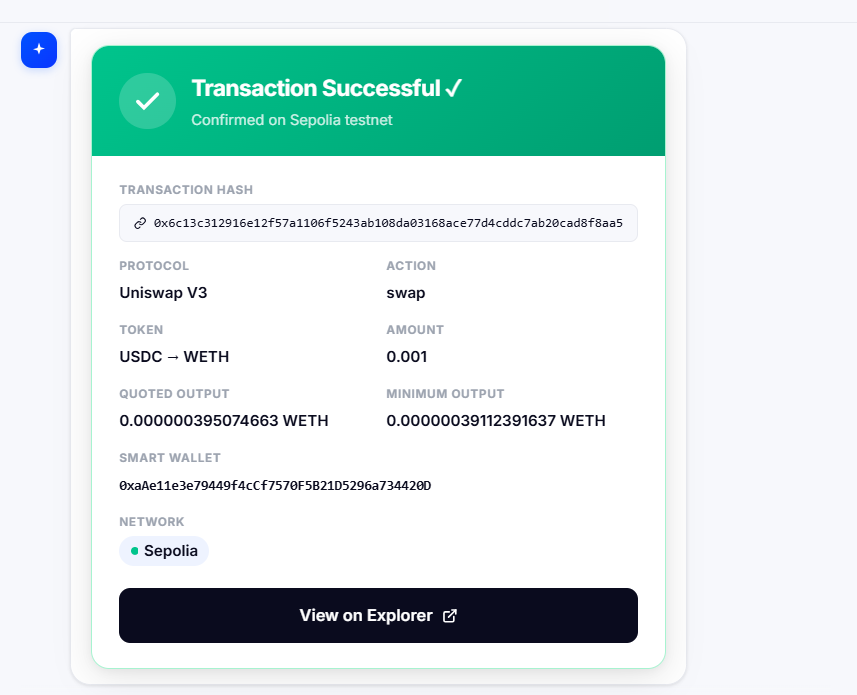
\includegraphics[width=0.95\linewidth]
        {figures/blockchain_execution.png}
    \caption{Transaction submission response for a
    Uniswap V3 swap on Ethereum Sepolia.}
    \label{fig:blockchain_execution}
\end{figure}

For Uniswap V3 swaps, the execution component obtains
quotes for the routes returned by the renewed graph
verification and selects the route with the highest
positive quoted output. The minimum acceptable output
is calculated using the stored slippage tolerance,
with a default of 100 basis points when no value
was specified. Before invoking
\texttt{exactInputSingle}, the component checks the
smart account's token balance and allowance. Where
necessary, the submitted call batch resets an existing
non-zero allowance and approves the required input
amount~\cite{implUniswapSingleSwap}.

For Aave V3, the execution component prepares supply,
withdraw, borrow, and repay calls using the verified
Pool contract and underlying asset~\cite{implAavePool}.
Borrowing and repayment use variable interest-rate
mode~2, and the referral code defaults to zero.
Supply operations check the available token balance,
while supply and repayment prepare the necessary
allowance changes. Dedicated checks for borrowing
capacity, collateral sufficiency, outstanding debt,
and lending-position constraints are not implemented.
Graph approval therefore does not establish that
the lending transaction will succeed.

The Kernel client submits the prepared operations.
When submission returns a transaction hash, the
backend reports \texttt{EXECUTED} with reason code
\texttt{TRANSACTION\_SUBMITTED}. This status indicates
submission through the wallet client, not confirmed
blockchain execution. Errors encountered during
preparation or submission produce \texttt{FAILED}.



The prototype does not independently reconcile
transaction receipts or post-execution balances.
Consequently, the execution response demonstrates
the implemented verification-to-submission handover,
but does not establish successful on-chain settlement.




\medskip
\noindent\textbf{Restricted Wallet Authorization.}
The execution component incorporates a custom
ERC-7579-compatible validator, \texttt{GraphBoundValidator},
to enforce restricted authorization through the
ERC-4337 smart-account validation mechanism. The authorization architecture separates the privileged
account owner, the verification authority, and the
restricted execution signer. Following graph re-verification,
the complete transaction batch is prepared and checked
against the retained approved operation. The verification
authority authorizes the exact encoded batch, including
contract destinations, callable functions, parameters,
and execution order. The restricted signer cannot
authorize modifications or additional calls without
a corresponding authorization from the verification
authority.

The validator enforces the smart-account and network
context, limited authorization validity, and single-use
approval identifiers. The mechanism was evaluated using
the actual ZeroDev Kernel and ERC-4337 EntryPoint
contracts in a local EVM environment. The tests
demonstrated successful authorization of all five
supported operation patterns and rejection of
unauthorized changes to execution parameters. The restricted authorization mechanism was not
deployed on public Ethereum Sepolia. Therefore,
public-bundler compatibility, testnet execution,
and production-level security remain unverified.



% ## 4.7 Summary ###

\section{Summary}
\label{sec:implementation_summary}

The prototype implements the proposed concept through distinct
stages of LLM-based intent generation, deterministic validation,
verification against maintained property-graph knowledge, and
controlled smart-wallet execution. Uniswap V3 swaps and Aave V3
supply, withdrawal, borrowing, and repayment are supported within
the configured Ethereum Sepolia context. Protocol-specific
knowledge acquisition and action-centred Cypher queries separate
language interpretation from the resolution of contracts, functions,
and protocol resources.

The implementation also reveals limitations in realizing the
conceptual guarantees. Knowledge synchronization requires external
invocation and is not fully atomic, while live Aave reserve
restrictions are only partially represented. Verification results
do not retain immutable evidence snapshots. Although the execution
endpoint repeats relationship verification, its comparison does not
bind every swap-preparation parameter to the original approval.
Wallet restrictions remain primarily application-level controls,
and the backend signer is not authenticated as the connected
browser account.

The following chapter evaluates intent processing, relationship
verification, knowledge maintenance, and the controlled execution
handover against the defined requirements.

